\documentclass[xetex,mathserif,serif]{beamer}
\usepackage{polyglossia}
\setdefaultlanguage[babelshorthands=true]{russian}
\usepackage{minted}
\usepackage{tabu}

\useoutertheme{infolines}

\usepackage{fontspec}
\setmainfont{FreeSans}
\newfontfamily{\russianfonttt}{FreeSans}

\usepackage{textpos}
\setlength{\TPHorizModule}{1cm}
\setlength{\TPVertModule}{1cm}

\definecolor{links}{HTML}{2A1B81}
\hypersetup{colorlinks,linkcolor=,urlcolor=links}

\tabulinesep=1.2mm

\title{Mock-объекты}
\author[Юрий Литвинов]{Юрий Литвинов\\\small{\textcolor{gray}{yurii.litvinov@gmail.com}}}
\date{27.02.2019г}

\newcommand{\attribution}[1] {
\vspace{-5mm}\begin{flushright}\begin{scriptsize}\textcolor{gray}{\textcopyright\, #1}\end{scriptsize}\end{flushright}
}

\begin{document}

	\frame{\titlepage}

	\begin{frame}
		\frametitle{Mock-объекты}
		\begin{itemize}
			\item Объекты-заглушки, симулирующие поведение реальных объектов и контролирующие обращения к своим методам
			\begin{itemize}
				\item Как правило, такие объекты создаются с помощью библиотек
			\end{itemize}
			\item Используются, когда реальные объекты использовать
			\begin{itemize}
				\item Слишком долго
				\item Слишком опасно
				\item Слишком трудно
				\item Для добавления детерминизма в тестовый сценарий
				\item Пока реального объекта ещё нет
				\item Для изоляции тестируемого объекта
			\end{itemize}
			\item Для mock-объекта требуется, чтобы был интерфейс, который он мог бы реализовать, и какой-то механизм внедрения объекта
			\begin{itemize}
				\item Как правило, как параметр конструктора или через поле
			\end{itemize}
		\end{itemize}
	\end{frame}

	\begin{frame}
		\frametitle{Пример}
		\begin{center}
			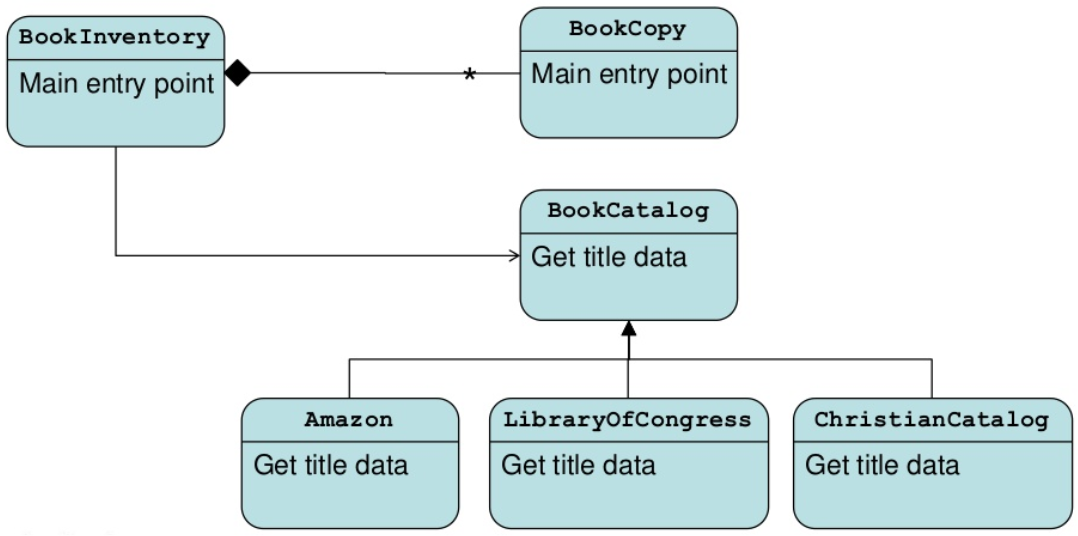
\includegraphics[width=0.9\textwidth]{classesHierarchy.png}
			\attribution{https://www.slideshare.net/sudharajamanickam/mockito-24306321}
		\end{center}
	\end{frame}

	\begin{frame}
		\frametitle{Объекты-заглушки}
		\begin{center}
			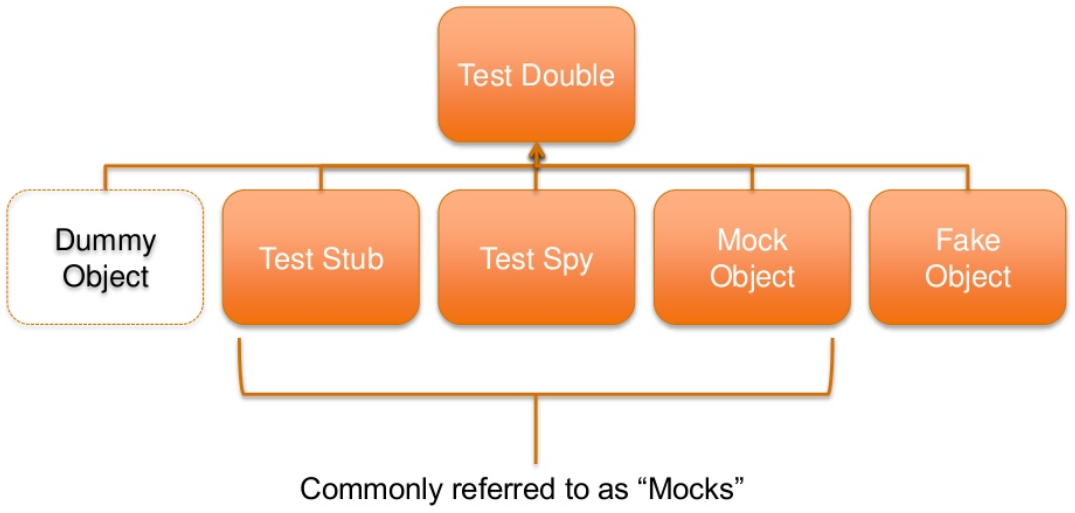
\includegraphics[width=0.9\textwidth]{testDoubles.png}
		\end{center}
		\url{http://tinyurl.com/testdoubles}
	\end{frame}

	\begin{frame}
		\frametitle{Stubs}
		\begin{itemize}
			\item Захардкоженные объекты, реализующие нужный интерфейс
			\item Наивная или вообще отсутствующая реализация
			\begin{itemize}
				\item Возможно какие-то assert’ы или полезная логика для теста
			\end{itemize}
		\end{itemize}
		\begin{center}
			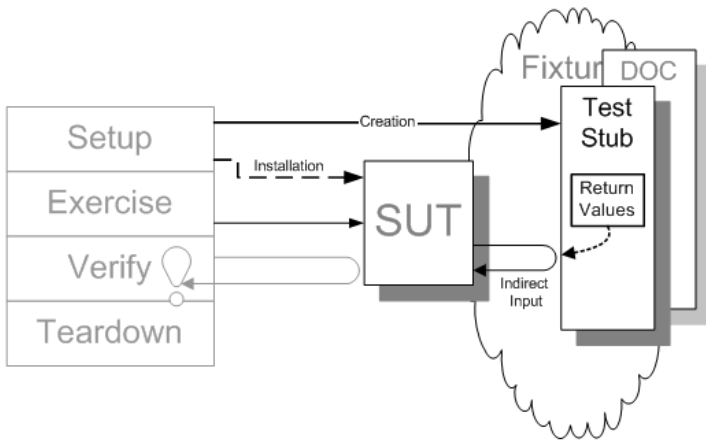
\includegraphics[width=0.6\textwidth]{stub.png}
			\attribution{http://xunitpatterns.com}
		\end{center}
	\end{frame}

	\begin{frame}
		\frametitle{Spies}
		\begin{itemize}
			\item Запуск теста, затем проверка условий и ограничений
		\end{itemize}
		\begin{center}
			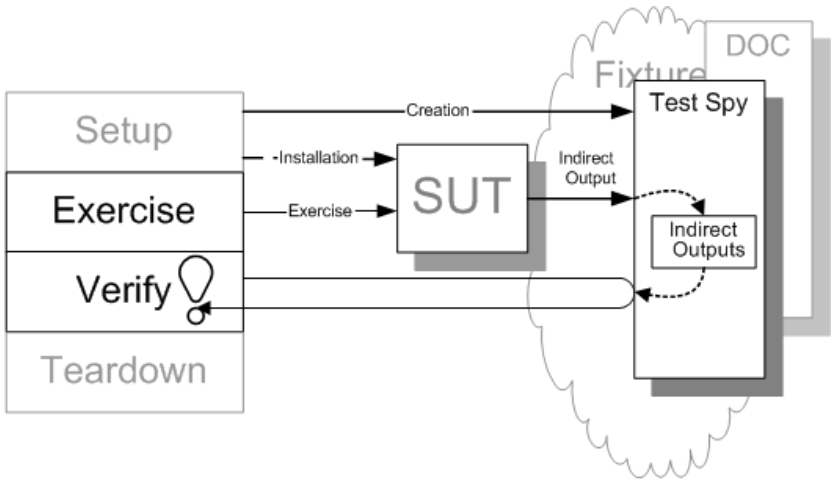
\includegraphics[width=0.6\textwidth]{spy.png}
			\attribution{http://xunitpatterns.com}
		\end{center}
	\end{frame}

	\begin{frame}
		\frametitle{Mocks}
		\begin{itemize}
			\item Конфигурирование объекта перед запуском теста
		\end{itemize}
		\begin{center}
			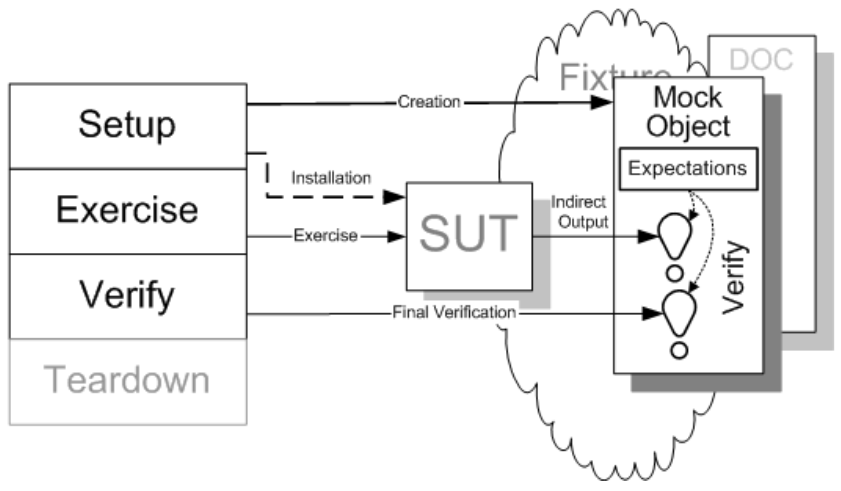
\includegraphics[width=0.6\textwidth]{mock.png}
			\attribution{http://xunitpatterns.com}
		\end{center}
	\end{frame}

	\begin{frame}[fragile]
		\frametitle{Классический тест}
		\begin{minted}{java}
@Test 
public void test() throws Exception {
    // Arrange
    var testee = new UnitToTest();
    var helper = new Helper();
    // Act
    testee.doSomething(helper);
    // Assert
    assertTrue(helper.somethingHappened());
}
		\end{minted}
	\end{frame}

	\begin{frame}
		\frametitle{Mockito}
		\begin{itemize}
			\item \url{http://site.mockito.org/}
			\item \url{https://github.com/mockito/mockito}
			\item MIT license
		\end{itemize}
	\end{frame}

	\begin{frame}[fragile]
		\frametitle{Тест с mock-объектом}
		\begin{minted}{java}
@Test
public void test() throws Exception {
    // Arrange, prepare behaviour
    Helper aMock = mock(Helper.class);
    when(aMock.isCalled()).thenReturn(true);
    // Act
    testee.doSomething(aMock);
    // Assert - verify interactions (optional)
    verify(aMock).isCalled();
}
		\end{minted}
	\end{frame}

	\begin{frame}[fragile]
		\frametitle{Создание mock-объектов}
		\begin{itemize}
			\item \mintinline{java}|IMyClass myMock = mock(IMyClass.class)|
			\pause
			\item \mintinline{java}|MyClass myMock = mock(MyClass.class)|
			\pause
			\item \mintinline{java}|@mock private MyClass myMock;|
			\begin{itemize}
				\item 
					\begin{minted}{java}
@Before public void setup() { 
    MockitoAnnotations.initMocks(this); 
}
					\end{minted}
			\end{itemize}
		\end{itemize}
	\end{frame}

	\begin{frame}[fragile]
		\frametitle{when(...)}
		\begin{itemize}
			\item \mintinline{java}|when(mock.someMethod()).thenReturn(10);|
			\pause
			\item 
				\begin{minted}{java}
when(mock.someMethod("some arg"))
    .thenThrow(new RuntimeException());
				\end{minted}
			\pause
			\item \mintinline{java}|when(mock.someMethod(anyString())).thenReturn(42);|
			\pause
			\item \mintinline{java}|when(mock.someMethod(anyInt())).thenReturn("element");|
			\pause
			\item 
				\begin{minted}{java}
when(mock.someMethod(argThat(list -> list.size() < 3)))
    .thenReturn(null);
				\end{minted}
			\pause
			\item 
				\begin{minted}{java}
verify(target, times(1)).receiveComplexObject(
    argThat(obj -> obj.getSubObject().get(0).equals("expected")));
				\end{minted}
		\end{itemize}
	\end{frame}

	\begin{frame}[fragile]
		\frametitle{Последовательные вызовы}
		\begin{itemize}
			\item 
				\begin{minted}{java}
when(mock.someMethod("some arg"))
    .thenThrow(new RuntimeException())
    .thenReturn("foo");
				\end{minted}
			\pause
			\item 
				\begin{minted}{java}
when(mock.someMethod("some arg"))
    .thenThrow(new RuntimeException())
    .thenReturn("foo");
				\end{minted}
			\pause
			\item \mintinline{java}|when(mock.someMethod(anyInt())).thenReturn("element");|
			\pause
			\item 
				\begin{minted}{java}
when(mock.someMethod("some arg"))
    .thenReturn("one", "two", "three");
				\end{minted}
			\pause
			\item Но:
				\begin{minted}{java}
when(mock.someMethod("some arg")).thenReturn("one")
when(mock.someMethod("some arg")).thenReturn("two")
				\end{minted}
		\end{itemize}
	\end{frame}

	\begin{frame}[fragile]
		\frametitle{Подмена действия}
		\begin{minted}{java}
when(mock.someMethod(anyString())).thenAnswer(new Answer() {
     Object answer(InvocationOnMock invocation) {
         Object[] args = invocation.getArguments();
         Object mock = invocation.getMock();
         return "called with arguments: " + args;
     }
 });
 
 //the following prints "called with arguments: foo"
 System.out.println(mock.someMethod("foo"));
		\end{minted}
	\end{frame}

	\begin{frame}[fragile]
		\frametitle{verify(...)}
		\begin{itemize}
			\item \mintinline{java}|verify(mock).someMethod();|
			\pause
			\item \mintinline{java}|verify(mock, timeout(100)).someMethod();|
			\pause
			\item 
				\begin{minted}{java}
verify(mock).someMethod(
    anyInt(), anyString(), eq("third argument"));
				\end{minted}
			\pause
			\item 
				\begin{minted}{java}
verify(mock).someMethod(
    argThat(someString -> someString.length() > 5));
				\end{minted}
		\end{itemize}
	\end{frame}

	\begin{frame}[fragile]
		\frametitle{Повторные вызовы}
		\begin{itemize}
			\item \mintinline{java}|verify(mock, times(2)).someMethod();|
			\pause
			\item \mintinline{java}|verify(mock, never()).someMethod();|
			\begin{itemize}
				\item \mintinline{java}|verifyZeroInteractions(mockTwo);|
			\end{itemize}
			\pause
			\item \mintinline{java}|verify(mock, atLeastOnce()).someMethod();|
			\pause
			\item \mintinline{java}|verify(mock, atLeast(2)).someMethod();|
			\pause
			\item \mintinline{java}|verify(mock, atMost(5)).someMethod();|
			\pause
			\item 
				\begin{minted}{java}
InOrder inOrder = inOrder(mock);
inOrder.verify(mock).someMethod("was called first");
inOrder.verify(mock).someMethod("was called second");
				\end{minted}
		\end{itemize}
	\end{frame}

	\begin{frame}[fragile]
		\frametitle{spy(...)}
		\begin{small}
			\begin{minted}{java}
List list = new LinkedList();
List spy = spy(list);

when(spy.size()).thenReturn(100);

spy.add("one");
spy.add("two");

//prints "one" - the first element of a list
System.out.println(spy.get(0));

//size() method was stubbed - 100 is printed
System.out.println(spy.size());

verify(spy).add("one");
verify(spy).add("two");
			\end{minted}
		\end{small}
	\end{frame}

	\begin{frame}[fragile]
		\frametitle{Hamcrest}
		\begin{itemize}
			\item \mintinline{java}|assertThat(someString, is(not(equalTo(someOtherString))));|
			\pause
			\item \mintinline{java}|assertThat(list, everyItem(greaterThan(1)));|
			\pause
			\item \mintinline{java}|assertThat(cat.getKittens(), hasItem(someKitten));|
			\pause
			\item \mintinline{java}|assertThat("test", anyOf(is("testing"), containsString("est")));|
			\pause
			\item 
				\begin{minted}{java}
assertThat(x, 
    allOf(greaterThan(0), lessThanOrEqualTo(10)));
				\end{minted}
		\end{itemize}
	\end{frame}

	\begin{frame}
		\frametitle{Примерное соотношение объёма тестов в проекте}
		\begin{center}
			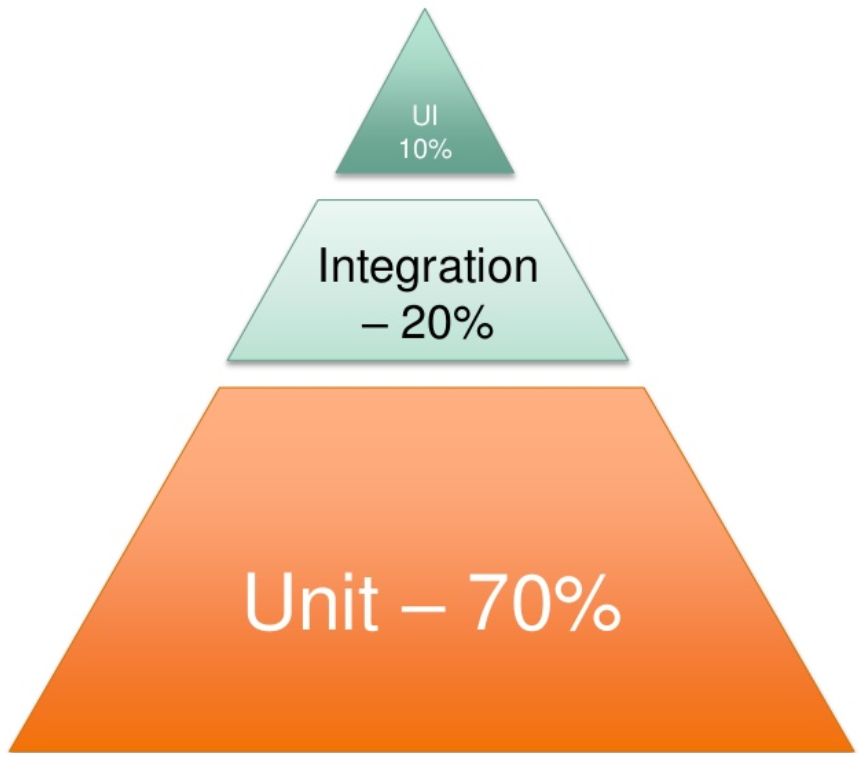
\includegraphics[width=0.6\textwidth]{testPyramid.png}
		\end{center}
	\end{frame}

	\begin{frame}
		\frametitle{Задание на остаток пары}
		\begin{itemize}
			\item Реализовать стековый калькулятор, принимающий на вход строку с арифметическим выражением в постфиксной записи и возвращающий результат его вычисления
			\begin{itemize}
				\item Должны поддерживаться операции $+$, $-$, $*$, $/$
				\item Можно использовать библиотечный стек
			\end{itemize}
			\item Протестировать калькулятор без стека с помощью библиотеки Mockito
		\end{itemize}
	\end{frame}

\end{document}
